%!TEX root = ../main.tex
%=========================================================

\vspace{-1mm}
\section{Introduction}
\vspace{-2mm}

With an average of 23,500 constantly live nodes~\cite{discv4-dns-lists}, the Ethereum ecosystem is one of the largest decentralized platforms currently in operation.
While it is widely known for supporting the blockchain of the same name (also known as the \emph{mainnet} and hosted by about 7,000 nodes), the platform is also home to a number of additional decentralized applications.
This includes blockchains used for test purposes (\emph{Ropsten}, \emph{G\"orli}), divergent blockchains resulting from a past fork (\emph{Ethereum classic}), alternative cryptocurrencies (\emph{Pirl}, \emph{Musicoin}), exchange markets (\emph{Binance}), content delivery networks (\emph{Swarm}), or messaging applications (\emph{Whisper}).
The platform already features almost 500 such applications, and their number grows every year~\cite{discv4-dns-lists}. The size distribution of the application-specific sub-networks varies significantly (\Cref{fig:ecosystem}) featuring a \emph{long tail}, with a vast majority of applications formed of a few hundred nodes or less.

\begin{figure}[t]
    \includegraphics[width=1\linewidth]{img/ecosystem}
    \vspace{-0.15in}
    \caption{Distribution of the number of nodes of Ethereum's sub-networks in May 2022, corresponding to different applications and sorted by decreasing popularity.
    A Zipf distribution is given for reference.
    }
    \vspace{-0.20in}
    \label{fig:ecosystem}
\end{figure}

All nodes in the Ethereum platform participate in a \emph{global} peer-to-peer (P2P) network operating a distributed hash table (DHT)~\cite{maymounkov2002kademlia}.
In addition to joining the global network, every node connects to at least one \emph{sub-network} formed of peers participating in its application(s) of interest.
In this paper, we focus on the \emph{service discovery} mechanism, by which a node participating in the global P2P network discovers this application sub-network.
Service discovery returns a set of peers that are used as entry points to that sub-network, typically supporting a specific overlay network as illustrated by \Cref{fig:subnetwork}.

\begin{figure}[b!]
    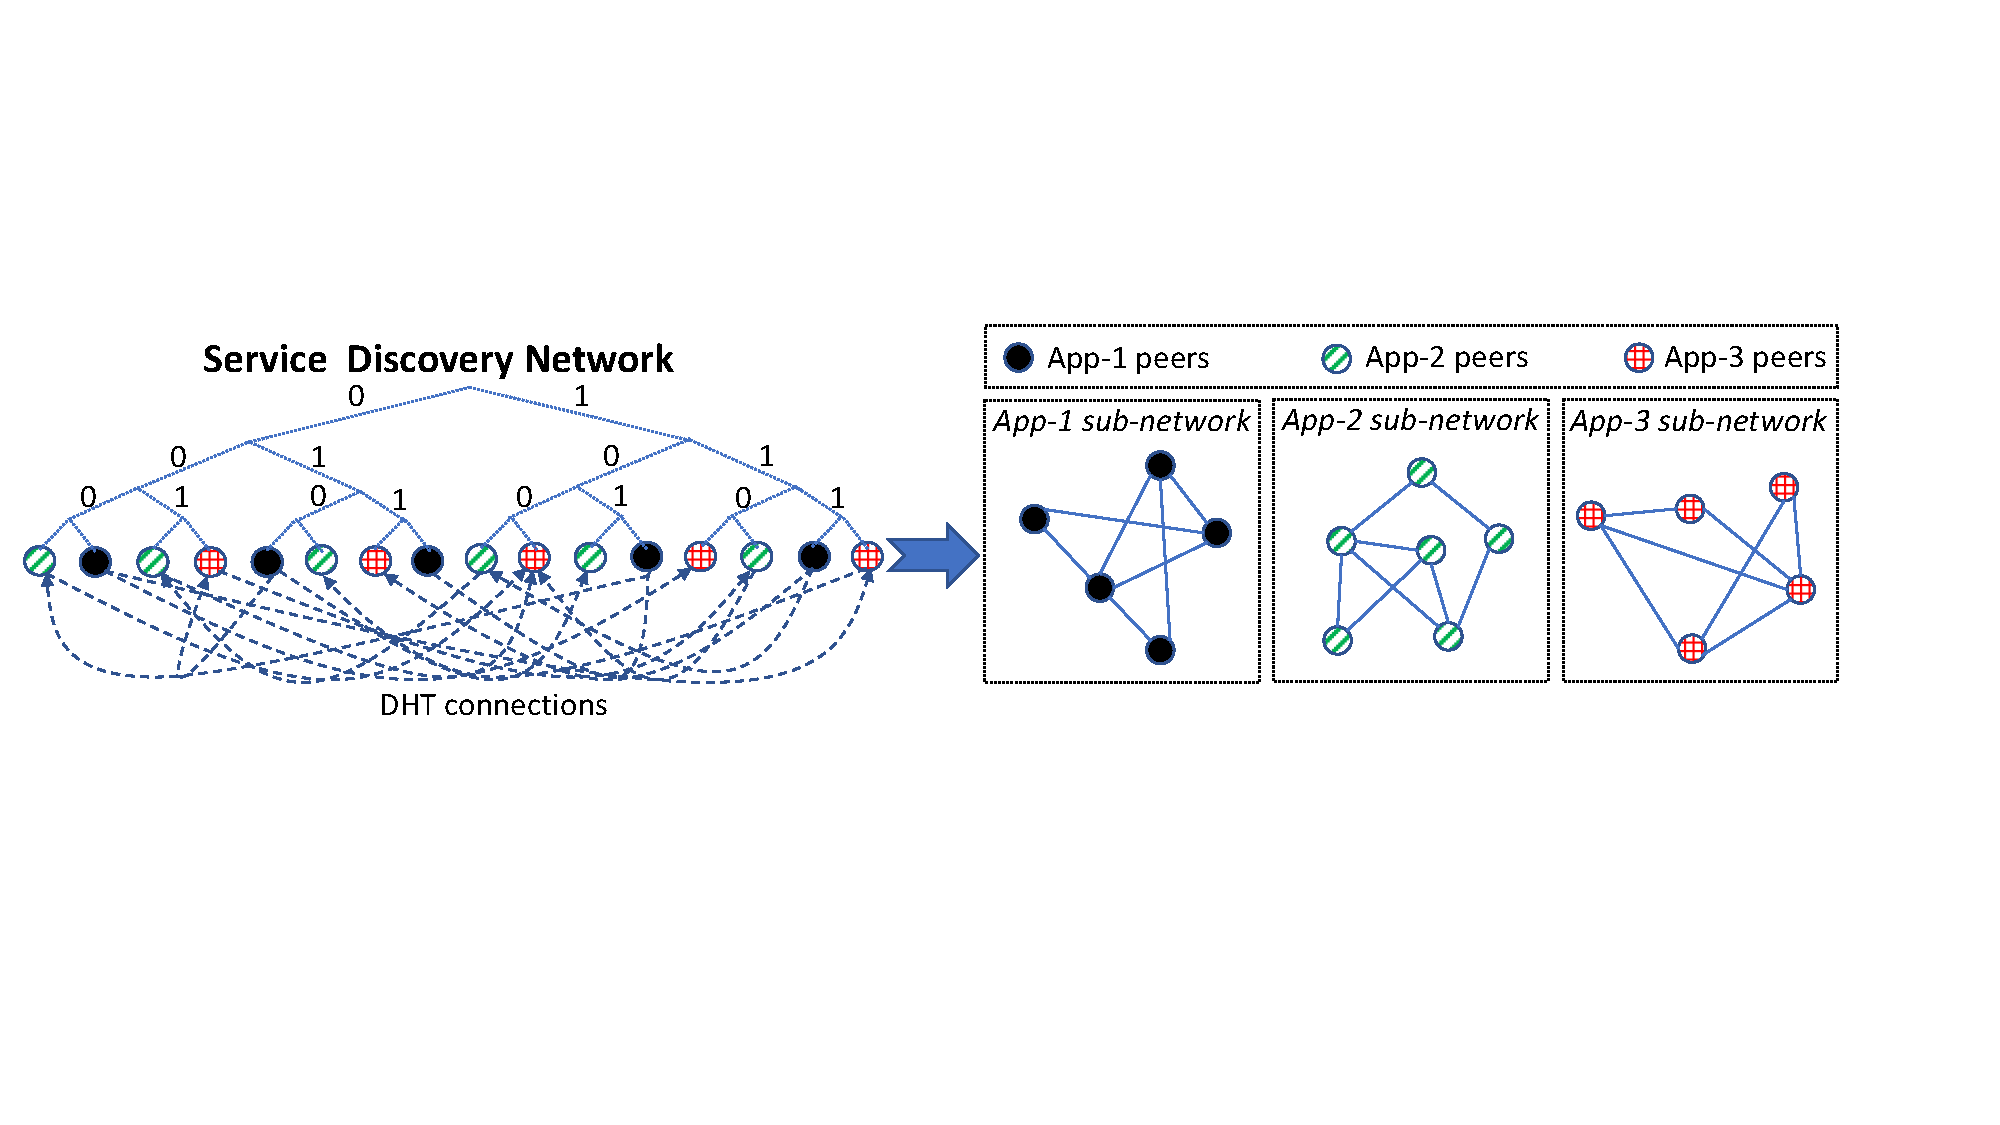
\includegraphics[width=1\linewidth]{img/subnetwork}
    \vspace{-0.15in}
    \caption{Formation of application-specific sub-networks using a universal service discovery network.
    \protect\er{would be good to have larger fonts in the figure, they are very small compared to those of Figure~\ref{fig:ecosystem}}
    }
    \label{fig:subnetwork}
    \vspace{-0.15in}
\end{figure}

Service discovery is a particularly sensitive mechanism in the Ethereum platform.
It must ensure that malicious participants to this open network are unable to bias its execution against a victim node or sub-network--and that, despite the ability of these adversaries to operate multiple Sybil identities.
Of particular importance is the protection against \emph{eclipse} attacks, where an adversary would lure its victim(s) into a sub-network formed of only nodes under its control.
Similarly, an adversary may run \emph{denial-of-service} attacks against a specific application, preventing other nodes from discovering peers from the associated sub-network.
On the other hand, the mechanism must remain efficient and scalable.
It is not desirable, for reasons of scalability and robustness, that it relies solely on fixed (sets of) dedicated registrar nodes maintaining the membership of each application.
Registrar nodes for popular applications could quickly become overwhelmed, and they would be an easy target for attackers.
In addition, the need to provision dedicated registrar nodes would be a hindrance to the emergence of new applications and (initially) small sub-networks.

% \er{There are inconsistencies with the presentation of discv4; here presented as a set of protocols but later as the name of the discovery mechanism itself. In general, we should clarify what are these other protocols. If these are helping/lower level protocols for the discovery mechanism I would prefer to present discv4 as the discovery mechanism (and do the same for discv5=\sysname).}
% \mk{Yes, we can to that (see the comments before the intro}

The current service discovery mechanism used in the Ethereum platform, named \discv~\cite{discv4}, leverages the global DHT for service discovery using a simple but robust \emph{random walk} approach.
A node willing to join an application's sub-network simply contacts individually a series of nodes collected from random lookups on the DHT, repeatedly checking application membership until it has collected enough peers participating in this target application.
This approach offers good resilience to malicious behaviors but it suffers from very poor scalability and performance, in particular for small sub-networks.
Random walks have, indeed, a decreasing likelihood of encountering peers from the target sub-network, increasing the number of messages required, join latency, and resource consumption at all the encountered peers.
% Our observations of \discv show that it can require no less than \hl{\textbf{XXX}} \er{FILL ME} attempts for a node to find \hl{\textbf{Y}} \er{FILL ME} different peers, for a medium-size sub-network already featuring \textbf{100} nodes, and significantly more for smaller sub-networks.
% \er{note that such numbers should be given also in the next section, so we may decide to cut the sentence here to avoid a repetition.}
As more applications join the DHT, the inefficiency of the random discovery process becomes a bottleneck for the entire ecosystem.
Alternative solutions for service discovery were proposed, but were meant for small-scale networks~\cite{zhang2002aggregate, helal2002standards}, centralised~\cite{RFC6763}, based on unrealistic assumptions~\cite{danezis2005sybil, danezis2009sybilinfer}, or insecure~\cite{baldoni2007tera,scribe,poldercast,banno2015,scribe}.
% We provide an extensive analysis of these systems in \Cref{sec:related}.

\smallskip
\noindent
\textbf{Contributions.}
%
We present in this paper \sysname, a novel service discovery mechanism for Ethereum.
\sysname targets a balance between robustness, i.e., the ability to resist malicious behaviors and Sybil identities, efficiency, i.e., fast service discovery even for small applications, and good load-balance over participating nodes.

After providing background knowledge and reviewing the current service discovery mechanism of Ethereum in \Cref{sec:background}, and detailing our system and threat models in \Cref{sec:model}, we detail \sysname as follows.

In \Cref{sec:placement}, we present how \sysname enables nodes, members of application sub-networks, to \emph{advertise} their membership to these applications in the form of \emph{service advertisements}.
Any node can act as a \emph{registrar} and store advertisements for any topic.
In contrast with the direct use of DHT lookups, however, in \sysname service advertisements propagate to a pseudo-random subset of all nodes in the global network.
The density of advertisements for an application increases as a service lookup approaches the key of a specific application in the DHT.

Robustness, load balancing, and efficiency for the discovery of smaller sub-networks all rely on a novel \emph{admission protocol}, by which registrars accept or reject incoming service advertisements (\Cref{sec:admission}).
It ensures that advertisers cannot effectively flood advertisements at a registrar, even when deviating from the protocol or operating Sybils, and that less popular topics get a sufficiently high probability to be represented and found.

At the core of our admission protocol lies the need for advertisers to respect a waiting time imposed by the registrars before being able to successfully register their advertisement.
We discuss the design and dynamics of the waiting function in \Cref{sec:waitingTime}.
The function allows limiting the amount of resources used by each node, promotes diversity of topic advertisements stored by each node, and protects against a vast range of malicious behaviors.

We summarize the results of the analysis of \sysname security in \Cref{sec:analysis}, and provide more thorough development of this analysis in \Cref{sec:appendix}.

\er{revise this paragraph in light of the deployment results; highlights could focus on real deployments.}
We overcome multiple practical challenges, implement \sysname in a simulator as well as in the code base of the \emph{Go Ethereum} (Geth) client~\cite{geth} (\Cref{sec:eval}).
Compared to \discv, \sysname discovers ten times more peers per time slot while achieving a similar or lower probability of being eclipsed by a powerful attacker.
Compared to vanilla DHT operations, our system eliminates vulnerability to attacks from resource-constrained attackers, and reduces load on the most busy node in the network by two orders of magnitude.
\sysname is currently being investigated by the Ethereum community for future use in the Ethereum ecosystem.

We finally review related work in \Cref{sec:related} and draw conclusions in \Cref{sec:con}.
 